\chapter{Preliminari}

\section{Diagrammi e tabelle}

\begin{defn}[Diagramma di Young]
Un diagramma di Young $\lambda=(n_1,n_2,\dots,n_k)$ \`e una
rappresentazione di una partizione di un intero positivo $n =
\sum_{i=0}^{k}{n_i}$ come somma di interi positivi $n_k \geq \ldots \geq
n_2 \geq n_1 \geq 0$. Graficamente possiamo rappresentare un diagramma di
Young come $k$ righe di celle quadrate, allineate a sinistra, di
lunghezza $n_k,\ldots,n_2,n_1$ dall'alto verso il basso in quest'ordine.
\end{defn}

\begin{defn}[Diagramma coniugato]
Dato un diagramma di Young $\lambda=(n_1,n_2,\dots,n_k)$, definiamo il
suo coniugato $\tilde{\lambda}$ come il diagramma che ha le colonne di
lunghezza $n_k,\ldots,n_2,n_1$ da sinistra verso destra in quest'ordine.  
\end{defn}

\begin{figure}[h]
\centering

\begin{subfigure}[b]{0.4\textwidth}
\centering
\includegraphics[height=0.35\textwidth]{YoungDiagram}
\caption{$\lambda=(1,1,2,3,4)$}
%% \label{fig:awesome_image}
\end{subfigure}%
\begin{subfigure}[b]{0.4\textwidth}
\centering
\raisebox{0.2\height}{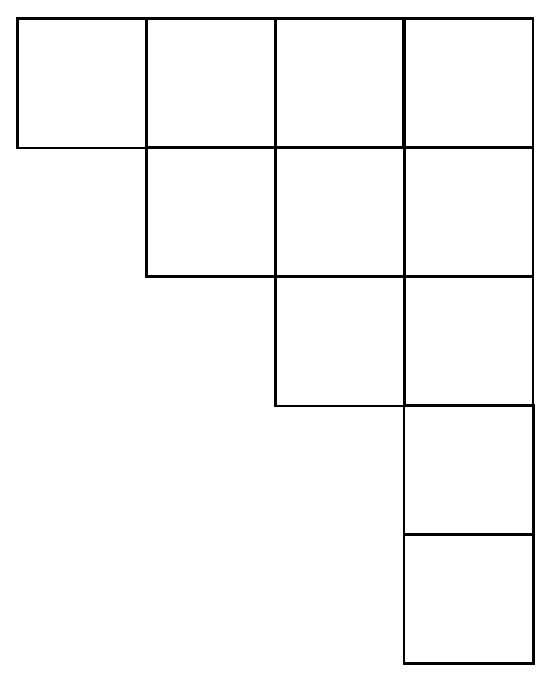
\includegraphics[height=0.35\textwidth,angle=90]{YoungDiagramFlip}}
\caption{$\tilde{\lambda}=(1,2,3,5)$}
\end{subfigure}
\caption{Un diagramma di Young ed il suo coniugato.}
\end{figure}

L'implementazione che abbiamo realizzato in Maxima di un diagramma di Young \`e
semplicemente una lista di interi positivi in ordine crescente.
La funzione \emph{remove\_diagram\_column} toglie la colonna pi\`u a
sinistra del diagramma e la inserisce come ultima riga del diagramma
coniugato. 
Dal momento che l'intero in posizione $i$-esima rappresenta
la lunghezza della riga $i$-esima del diagramma, togliere una colonna
equivale a diminuire di uno ogni elemento della lista, e
nell'eventualit\`a che si ottenga uno zero in prima posizione,
significa che abbiamo tolto abbastanza colonne da aver eliminato la
prima riga del diagramma.

Ad esempio, in Maxima possiamo ottenere il diagramma coniugato di
$\lambda=(1,1,2,3,4)$ con la nostra funzione
\begin{alltt}
\emph{ydiagram\_transpose\_rows} ([1,1,2,3,4]);
\(\rightarrow\) [1,2,3,5]
\end{alltt}

%% \begin{figure}[h]
%% \centering
%% 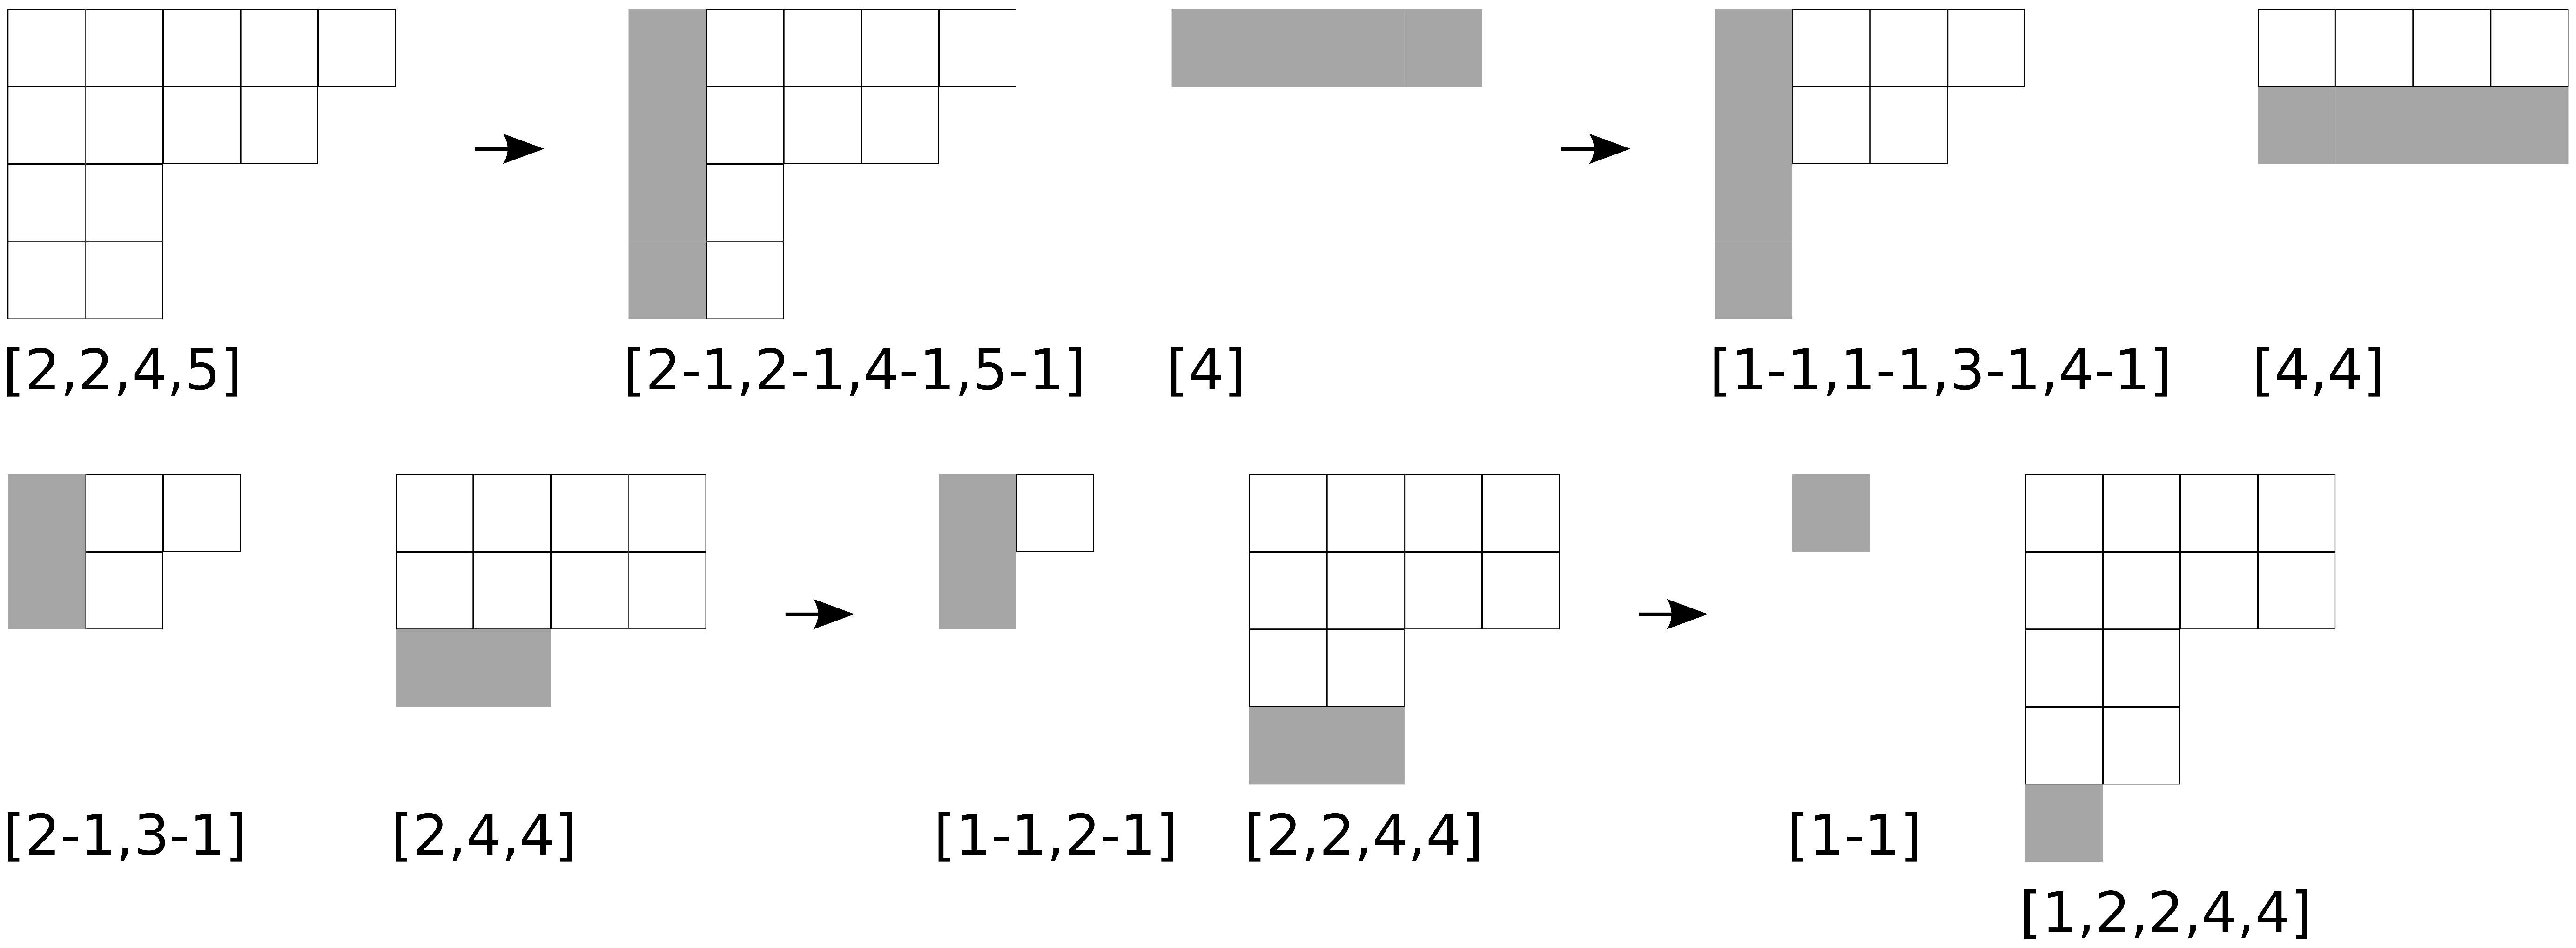
\includegraphics[width=1\textwidth]{transpose_diagram}
%% \caption{Trasposizione di un diagramma di Young}
%% \label{fig:transpose_diagram}
%% \end{figure}

\begin{notaz}
Scriveremo $\lambda \vdash n$ intendendo che $\lambda$ \`e una
partizione di $n$.
\end{notaz}

\begin{defn}
Diremo che un diagramma $\mu=(n_1,n_2,\dots,n_k)$ \emph{\`e pi\`u
piccolo} di un diagramma $\lambda=(m_1,m_2,\dots,m_h)$, e scriviamo
$\mu \subset \lambda$, se
\begin{enumerate}[(i)]
\item $k \leq h$;
\item $n_i \leq m_i$ per ogni $1 \leq i \leq k$.
\end{enumerate}
\end{defn}

\begin{defn}[Tabella di Young]\label{ytab}
Diremo Young tableau un riempimento di un diagramma di Young con
numeri interi positivi che risulti:
\begin{enumerate}[(i)]
\item non decrescente lungo le righe;
\item strettamente crescente lungo le colonne.
\end{enumerate}
Un Young tableau si dice \emph{standard} se il riempimento di
$\lambda \vdash n$ \`e composto dai primi $n$ interi positivi (non
ripetuti).
\end{defn}

\begin{oss}
Un Young tableau standard \`e strettamente crescente \emph{anche}
lungo le righe.
\end{oss}

\begin{oss}
Ogni tabella $T$ \`e riempimento di un unico diagramma $\lambda$. Il
diagramma di cui $T$ \`e riempimento \`e detto \emph{forma di $T$}.
\end{oss}

\begin{defn}[Skew diagram]
Uno skew diagram \`e il diagramma che si ottiene togliendo a
diagramma di Young $\lambda$ un diagramma pi\`u piccolo $\mu \subset
\lambda$. Indicheremo lo skew diagram cos\`i ottenuto con $\lambda / \mu$.
\end{defn} 

\begin{defn}[Skew tableau]
Diremo skew tableau un riempimento di uno skew diagram che rispetti i
requisiti della definizione \ref{ytab}. 
\end{defn}

Rappresentiamo in Maxima i tableaux come liste di liste di lunghezza
non decrescente, ognuna delle quali rappresenta una riga del tableau.
La struttura \`e riempita rispettando le condizioni della definizione.
Sfruttando la struttura che implementare i tableaux, realizziamo gli
skew diagram $\lambda/\mu$ come dei tableaux contenenti i simboli $0$ e $\infty$.
Usiamo $0$ per rappresentare una posizione ``proibita'', ovvero una
posizione contenuta sia nel diagramma $\lambda$ che nel diagramma
$\mu$, mentre usiamo $\infty$ per una posizione contenuta nel
diagramma $\lambda$ ma non in $\mu$ che quindi fa effettivamente parte
dello skew diagram. Dati due diagrammi possiamo calcolare lo skew
diagram attraverso la funzione\\
\texttt{\emph{generic\_skew\_tableau} (rev\_big\_shape,rev\_small\_shape,gen\_skew\_tab,curr)}.
Ad esempio per calcolare lo skew diagram $\lambda / \mu$ originato da
$\lambda=(2,3,4,5)$ e $\mu=(1,3,3)$

\begin{alltt}
\emph{generic\_skew\_tableau} (reverse ([2,3,4,5]),reverse ([1,3,3]),[],1);
\(\rightarrow [[\infty,\infty],[0,\infty,\infty],[0,0,0,\infty],[0,0,0,\infty,\infty]]\)
\end{alltt}

\section{Row bumping}\label{rowbump_par}
Il row bumping \`e la procedura con la quale dati un tableau $T$ e un
intero positivo $x$ si costruisce un tableau, che indicheremo con $T
\gets x$, la cui forma ha un box in pi\`u della forma di $T$ con
entrata $x$ (Figura \ref{fig:rowbump}).

\begin{figure}[h]
\centering
\includegraphics[width=0.8\textwidth]{row_bump}
\caption{Row bumping}
\label{fig:rowbump}
\end{figure}

Sia $x_1 = x$ l'elemento da inserire nel tableau $T$, se $x_1$ \`e non 
minore di ciascun elemento della prima riga
dall'alto di $T$, aggiungiamo alla fine di tale riga l'entrata x.
Altrimenti se $x_2$ \`e il primo elemento da sinistra della prima riga
di $T$ strettamente maggiore di $x_1$, inseriamo $x_1$ al posto di
$x_2$ e procediamo al suo inserimento nella seconda riga di $T$.
Ripetiamo quindi per le successive righe, fino a quando non siamo in
grado di effettuare un inserimento al termine di una riga oppure fino
a quando aggiungeremo una riga in basso contenente l'elemento $x_h$
sostituito nell'ultima riga al passo precedente con l'elemento
$x_{h-1}$.
Abbiamo implementato \texttt{\emph{rec\_bump\_row} (r,x,i)} che effettua il row bumping di un dato
elemento $x$ in una riga $r$ scorrendola dal fondo (chiameremo infatti
la funzione con $i$ pari alla lunghezza della riga) fino a trovare
l'elemento da sostituire oppure aggiungendo una nuova entrata in coda.
Restituisce la riga modificata con, eventualmente, l'elemento da
inserire nella riga successiva.

La funzione \texttt{\emph{rec\_ytableau\_word\_bump} (t,x,i)}, dove
$t$ \`e un tableau, $x$ \`e l'elemento che stiamo inserendo e $i$ il
numero di righe del tableau, esegue il row bumping
fino a quando \`e possibile, e se necessario aggiunge una nuova riga
al tableau $t$. Ad esempio possiamo ottenere il risultato mostrato in
figura \ref{fig:rowbump} con

\begin{alltt}
\emph{rec\_ytableau\_word\_bump} ([[7],[6,8],[4,7,7],[2,4,5,6],[1,1,2,5]], 1, 5)
\(\rightarrow\) [[7,8],[6,7],[4,4,7],[2,2,5,6],[1,1,1,5]]
\end{alltt}

\begin{oss}
Al termine di ogni iterazione della funzione
\emph{rec\_ytableau\_word\_bump} la variabile $t$ \`e la parola di un
tableau. In particolare la funzione \emph{rec\_ytableau\_word\_bump}
restituisce uno Young tableau.
%% \begin{proof}
%% Infatti la funzione \emph{rec\_bump\_row} restituisce una lista
%% ordinata in modo non decrescente (da sinistra verso destra), che
%% quindi rispetta la prima propriet\`a della definizione \ref{ytab}.\\
%% Supponiamo ora che al termine di una certa iterazione smetta di valere la seconda
%% propriet\`a, ovvero stiamo inserendo nella posizione
%% $(i,j)$ un intero $x$ minore o uguale dell'elemento $\bar{x}$ in
%% posizione $(i-1,j)$.\\
%% Durante l'iterazione precedente si \`e quindi inserito $y$ al posto di
%% $x$ nella riga $(i-1)$-esima, e poich\`e $x \leq \bar{x}$ tale
%% inserimento deve essere avvenuto (per la (i) della definizione
%% \ref{ytab}) in posizione $(i-1,k)$, con $k \leq j$. Sia $x_0$
%% l'elemento in posizione $(i,k)$, allora $x < x_0$.\\
%% Siamo quindi giunti ad un assurdo, infatti un tale inserimento
%% contraddice la non decrescenza. 
%% \end{proof}
\end{oss}

Iterando l'operazione di row bumping (figura \ref{fig:tab_prod}) si ha la seguente

\begin{defn}
Dati due tableaux $T$ e $U$, dette $x_1,\ldots , x_s$ le entrate di
$U$ da sinistra verso destra e dal basso verso l'alto, definiamo
$T \cdot U = (( \ldots ((T \gets x_1) \gets x_2 ) \gets \ldots ) \gets x_{s-1} )
\gets x_s$.
\end{defn} 

\begin{figure}[h]
\centering
\includegraphics[width=1\textwidth]{tableaux_product}
\caption{Prodotto di due tableaux}
\label{fig:tab_prod}
\end{figure}

\begin{oss}
Il prodotto di tableaux non \`e commutativo, infatti ad esempio
\begin{center}
\includegraphics[width=0.3\textwidth]{prod_non_comm_oneline}
\end{center}
\end{oss}

\section{Algebra dei tableaux}

\begin{prop}\label{tableaux_monoid}
L'insieme dei tableaux con l'operazione di prodotto \`e un monoide con
unit\`a data dal tableau vuoto che indichiamo con $\varnothing$.
\end{prop}

La dimostrazione di questo fatto richiede l'introduzione di alcuni
concetti.

\begin{defn}[Parola]
Dato un tableau o uno skew tableau $T$, diciamo row word, word o parola
di $T$, che indicheremo con $w(T)$, la parola che si ottiene elencando
da sinistra verso destra, dal basso verso l'alto le entrate di $T$.
\end{defn}

Ad esempio la parola associata al tableau ottenuto nel prodotto di
figura \ref{fig:tab_prod} \`e $87766447225511123$.

\begin{alltt}
\emph{word\_from\_ytableau} ([],[[8],[7,7],[6,6],[4,4,7],[2,2,5,5],[1,1,1,2,3]])
\(\rightarrow\) [8,7,7,6,6,4,4,7,2,2,5,5,1,1,1,2,3]
\end{alltt}

\begin{oss}
Dalla parola $w(T)$ di un tableau \`e possibile risalire al tableau
$T$ osservando che le righe di $T$, dal basso verso l'alto, si
ottengono leggendo la parola da sinistra verso destra e interrompendo
ogni volta in cui una lettera \`e strettamente minore della
precedente.
\begin{alltt}
\emph{ytableau\_from\_word} ([8,7,7,6,6,4,4,7,2,2,5,5,1,1,1,2,3], [])
\(\rightarrow\) [[8],[7,7],[6,6],[4,4,7],[2,2,5,5],[1,1,1,2,3]]
\end{alltt}
\end{oss}

\begin{notaz}
Se $u$ e $v$ sono due parole, scriviamo $u \leq v$ se ogni
\emph{ogni} lettera che occorre in $u$ \`e minore o uguale di \emph{ogni} lettera
che occorre in $v$. Se invece $u$ \`e una parola e $x$ un intero
positivo scriviamo $u \leq x$ se ogni lettera che occorre in $u$ \`e
minore o uguale di $x$. Analogamente per le disuguaglianze inverse e quelle in senso stretto. 
\end{notaz}

La cosa interessante \`e l'effetto del row bumping sulla
parola di un tableau. 
Possiamo interpretare l'algoritmo che descrive
il row bumping in termini di parole: sia $w = w(T)$ la parola in questione e
$x$ l'elemento da inserire. Possiamo fattorizzare $w=\bar w (u \bar x
v)$ dove $\bar w$ \`e la parola del tableau ottenuto da $T$ rimuovendo
la prima riga e $u \bar x v$ \`e la parola corrispondente
alla prima riga di $T$, dove $u$ \`e composta da lettere non maggiori
di $x$ e $\bar x > x$. Si ha $w \cdot x = \bar w \bar x u x
v$. Cio\`e:

\begin{equation}\label{row_bump_word}
u \bar x v \cdot x = \bar x u
  x v \mbox{ se } u \leq x < \bar x \leq v
\end{equation}

Infatti se $v=v_1 \ldots v_k$ la \eqref{row_bump_word}, tenuto conto che
$x < \bar x \leq v_i$ per ogni $1 \leq i \leq k$, diventa

\begin{equation}\label{pre_bump}
\begin{split}
u \bar x (v_1 \ldots v_k \cdot x)
= u \bar x (v_1 \ldots v_{k-1}
\cdot x )v_k = \ldots\\
\ldots = u \bar x (v_1 \ldots
v_i \cdot x )v_{i+1} \ldots v_k = \ldots
= u \bar x x v_1 \ldots v_k
\end{split}
\end{equation}

inoltre detto $u=u_1 \ldots u_h$, dato che $u_i \leq x < \bar x$, possiamo
descrivere il bumping di $\bar x$ come

\begin{equation}\label{bump}
\begin{split}
(u_1 \ldots u_k \cdot \bar x) x v
= (u_1 \ldots u_{h-1} \cdot \bar x) u_k x v = \ldots\\
\ldots =  (u_1 \ldots u_i \cdot \bar x
)u_{i+1} \ldots u_h x v = \ldots
= \bar x u_1 \ldots u_h x v.
\end{split}
\end{equation}

Possiamo quindi identificare due trasformazioni fondamentali: la prima
viene applicata a tre lettere consecutive ad ogni passaggio in \eqref{pre_bump}, la seconda
in \eqref{bump}:

\begin{equation}\label{k1}\tag{$K_1$}
y z x = y x z \mbox{ se } x < y
\leq z
\end{equation}
\begin{equation}\label{k2}\tag{$K_2$}
y z x = z y x \mbox{ se } y
\leq x < z
\end{equation}

\begin{defn}[Trasformazione elementare di Knuth]
Una trasformazione di una parola si dice elementare di Knuth se
applica a tre lettere consecutive la trasformazione \eqref{k1} o la
\eqref{k2}.
\end{defn}

\begin{defn}[Knuth-equivalenti]
Due parole $w$ e $w'$ si dicono Knuth-equivalenti, e si scrive $w
\equiv w'$ se \`e possibile ottenere una dall'altra per mezzo di una catena di
sole trasformazioni elementari di Knuth.
\end{defn}
%% \newpage % tornava brutto con l'immagine alla pagina dopo
\begin{oss}
Le trasformazioni fondamentali \eqref{k1} e \eqref{k2} sono coerenti
con il row bumping, infatti

\begin{figure}[h]
\centering
\begin{subfigure}[b]{0.3\textwidth}
\centering
\includegraphics[height=0.2\textwidth]{KnuthK1}\\
\eqref{k1} $x < y \leq z$
%% \label{fig:awesome_image}
\end{subfigure}%
\begin{subfigure}[b]{0.3\textwidth}
\centering
\includegraphics[height=0.2\textwidth]{KnuthK2}\\
\eqref{k2} $y \leq x < z$
\end{subfigure}
\caption{Trasformazioni fondamentali}
\end{figure}
\end{oss}
\FloatBarrier

\begin{prop}\label{word_bump_equiv}
Siano $T$ un tableau e $x$ un intero positivo, allora $w(T \gets x) = w(T)
\cdot x$. In particolare, dato un altro tableau $U$ si ha $w(T\cdot U)
= w(T) \cdot w(U)$.
\end{prop}

Data una parola $w = x_1 \ldots x_k$ possiamo sempre costruire un
tableau, per mezzo di quella che viene detta \emph{procedura canonica}
calcolando $T = (( \ldots ((\varnothing \gets x_1) \gets x_2 ) \gets \ldots ) \gets x_{k-1} )
\gets x_k$. Il tableau ottenuto ha parola $w(T)$ Knuth-equivalente a
$w$.

\begin{teo}\label{knuth_equiv_word}
Ogni parola \`e Knuth-equivalente alla parola di un unico tableau.
\end{teo}

Osservando che la giustapposizione di parole \`e associativa, si ha
infine la proposizione \ref{tableaux_monoid}.
